\documentclass[11pt]{article}
\usepackage[margin=1in]{geometry}
\usepackage{amsthm, amsmath, amssymb, mathtools}
\usepackage{graphicx}
\usepackage{tabularx}
\usepackage{caption}
\usepackage{pdfpages}

\title{DOT Summary}

\begin{document}
\maketitle

This document describes the data that is available in each edition of the Dictionary of Occupational Titles (DOT). The DOT provides job descriptions for thousands of jobs and was meant to be used as a tool for matching job seekers to jobs. The descriptions include information regarding the industry and occupation group the job is in. In each edition, jobs are assigned a hierarchical occupation code. In this code, the first digit describes the broad occupation group. For example, codes starting with 0 correspond to professional and managerial occupations. The successive digits of the code add more detail (e.g. codes starting with 07 correspond to managerial occupations). The codes for occupation groups can change over time and occupations are added and deleted as work is created or becomes obsolete. We are currently trying to see if there is a complete crosswalk between DOT occupations and Census occupations. We are also trying to find a digitized file with the title changes between different editions of the DOT. 

\section*{First Edition, 1939}

This edition has 29,000 job titles and 17,542 defined occupations. The occupations are coded using 5 or 6 digit codes. The occupational definition is a brief description of what the job entails and includes what industries the occupation is in. Part 4 of this edition contains very detailed matching criteria for entry level job seekers (personal traits, leisure time activities, casual work experience, and training courses). Each criteria (e.g. leisure time of tinkering with radios) is matched to an entry level occupation deemed to be a good fit. This detailed matching criteria is only available for entry level occupations.

\section*{Second Edition, 1949}

This edition has 40,000 job titles and 22,028 defined occupations. There are 7 major occupation groups, and about 1,000 3-digit occupation groups, each of which contains one or more occupations. The occupational definition is a brief description of the job duties and includes what industries the occupation is in.

\section*{Third Edition, 1965}

This edition has 35,500 titles and 21,741 defined occupations. There are two arrangements in this edition, the occupational group arrangement and the worker trait arrangement. Each occupation is described with a 6-digit code. The last 3 digits of the code describe the degree to which the job deals with data, people, and things. The first volume has the occupational group arrangement and the second volume has the worker trait arrangement. Both are described below.

\subsection*{Occupational Group Arrangement}
In this arrangement, the job titles are arranged by occupation group. There are 9 broad occupational categories (e.g. professional, clerical), which are subdivided into 84 2-digit divisions (e.g. stenography, styping). The divisions, in turn, are subdivided into 603 3-digit groups. The job definition in this arrangement includes what gets done, how it gets done, and why it gets done, as well as the industries it's done in.

\subsection*{Worker Trait Arrangement}
In this arrangement, the job titles are arranged by the job task requirements in the form of the 3 digit code that describes the level of involvement with data, people and things. In this arrangement, the definition includes the work performed, worker requirements, indications for relating applications and requirements, training, and methods of entry. The definition also has general educational development, specific vocational preparation, aptitudes, interests, temperaments, and physical demands.

\section*{Fourth Edition, 1977}
This edition has 20,000 defined occupations. Occupations are coded with 9-digit codes. The first 6 digits of this code are the same as in the previous edition. The last 3 digits of the code were added so that each title has a unique code. The job definition includes the industry and a brief description of the job. A supplement to this edition includes every job's physical demands, environmental conditions, required math and language development, and required specific vocational preparation.


\section*{Revised Fourth Edition, 1991}
This edition has the same information as the fourth edition, but with about 1,000 additional occupations.

\begin{table}[!htbp]
  \caption{Data available in each year}
  \begin{tabular}{lllllllllll}
       & \#of Definitions     & Interests & Aptitudes & Temperatments & DPT & Physical & Math & Language & SVP \\
  1939 & 17,500  &       &    &    &         &          &    &  &   &  \\
  1949 & 22,000    &      &    &    &        &          &     &  &   &  \\
  1965 & 21,700   &   \checkmark    &  \checkmark  &   \checkmark &  \checkmark       &   \checkmark       &  \checkmark   & \checkmark  &  \checkmark &  \\
  1977 & 20,000    &       &    &    &   \checkmark  &   \checkmark       &  \checkmark   & \checkmark  &  \checkmark &  \\
  1991 & 21,000 &   \checkmark    &  \checkmark  &   \checkmark &  \checkmark       &   \checkmark       &  \checkmark   & \checkmark  &  \checkmark &

  \end{tabular}
  \bigskip
Note: DPT is data, people, things and SVP is specific vocational preparation. One occupation can appear under different titles, but there is a one to one correspondence between occupations and definitions.
\end{table}

\section*{Features and Missing Data}
Detailed information regarding aptitudes and interests was collected for the Fourth Edition but was not published. We are working on acquiring that data.
Below is a list of all the available features for the Revised Fourth Edition. The worker functions, training times, aptitudes, and physical demands variables are also available for the Third Edition, but would need to be digitized.
There are temperaments and interests variables in the Third Edition, but they are very different from those in the Revised Fourth Edition and likely incomparable.

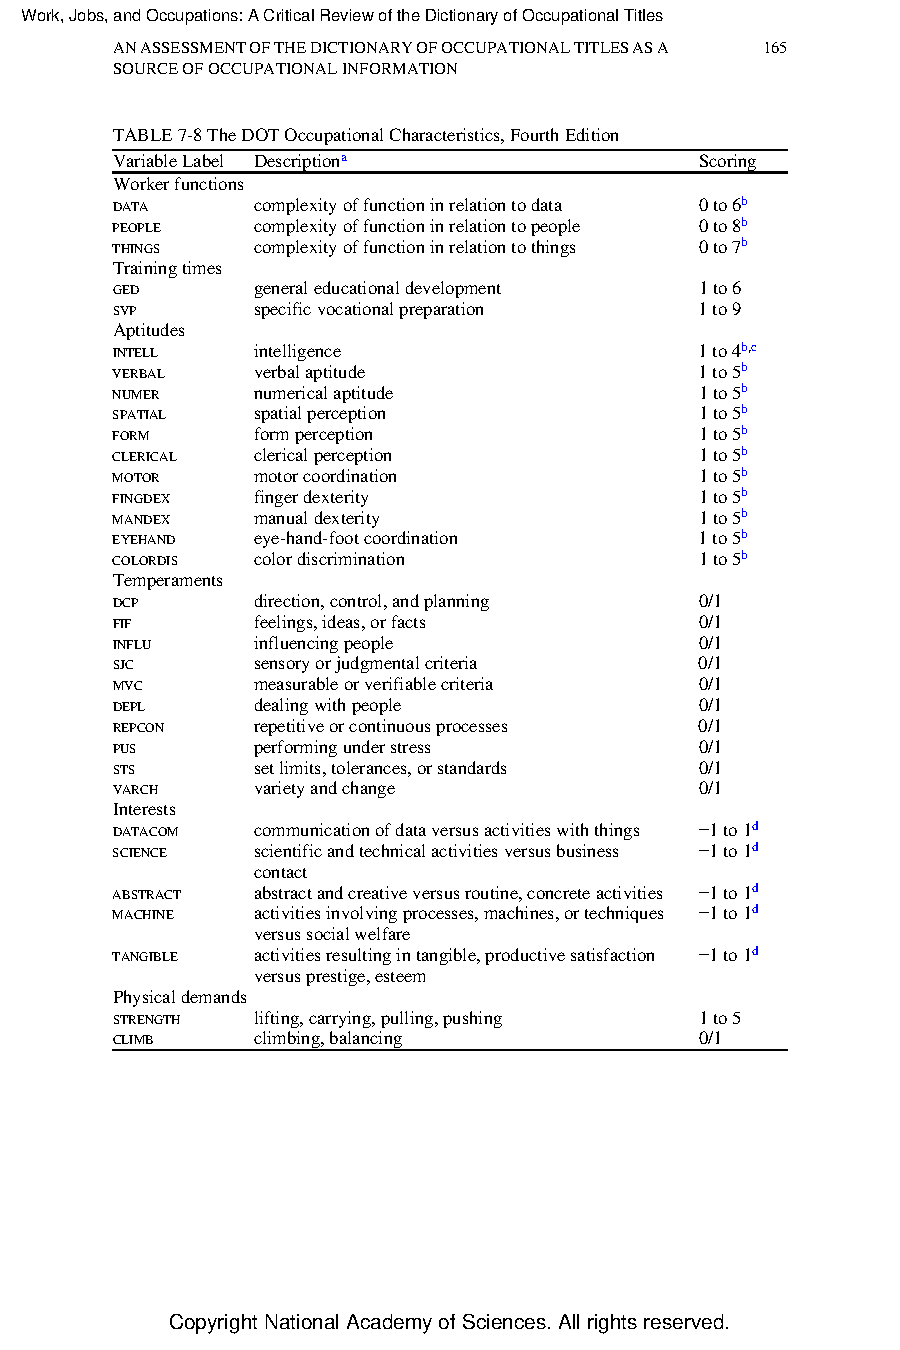
\includepdf[page=-]{job_features}

\end{document}
